%   Filename    : chapter_4.tex 

\chapter{Results and Discussions}

This chapter presents the results from the machine learning and deep learning analyses conducted on the preprocessed dataset. It includes an evaluation of various machine learning classifiers and the application of deep learning models for image-based classification. The primary focus is on identifying key predictors and assessing classification performance for sex identification in \textit{T. granosa}.

\section{Machine Learning Analysis}
This chapter outlines the results of preprocessing, training of machine learning models, and feature importance analysis, all conducted in Google Colab using Python. The dataset was preprocessed in Colab, and the training and evaluation of various classifiers were performed entirely within this environment.  This part of the paper includes five subsections: data exploration, statistical analysis, feature importance analysis, performance evaluation, and confusion matrix analysis.

\subsection{Data Exploration}

\begin{figure}[!htbp]
	\centering
	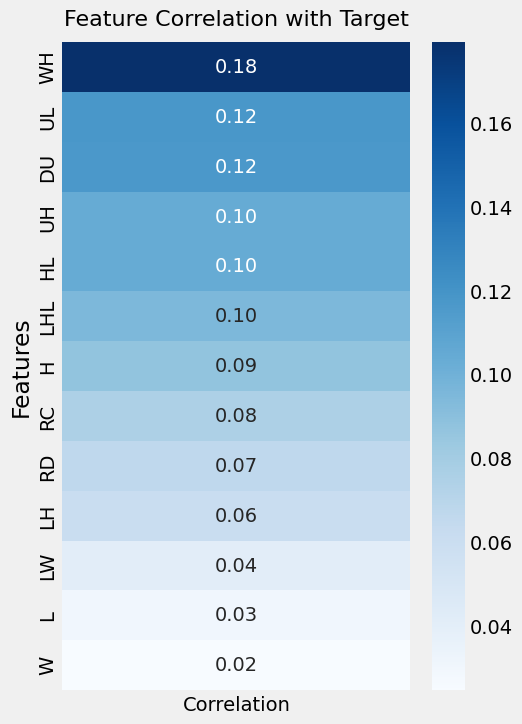
\includegraphics[width=0.4\textwidth]{figures/heatmap.png}
	\caption{Correlation heatmap of morphometric features with the sex of \textit{T. granosa}}
	\label{fig:heatmap}
\end{figure}

Exploratory data analysis was performed to characterize the dataset using visualizations to understand the patterns and correlations within the data. A correlation heatmap was created to assess the relationship between the predictors and the target variable.

The heatmap (see Figure~\ref{fig:heatmap}) revealed three features most correlated with the sex of \textit{T. granosa}: the width-height ratio (r = 0.18), the umbos-length ratio (r = 0.12), and the distance between the umbos (r = 0.12). Each of these features demonstrated a weak positive relationship with the target variable. 

\subsection{Statistical Analysis}

\begin{table}[H]
	\centering
	\small % or \footnotesize or \scriptsize
	\begin{tabular}{lc}
		\hline
		\textbf{Variable} & \textbf{p-value} \\ \hline
		Length & 0.334 \\
		Width & 0.753 \\
		Height & 0.124 \\
		Rib count & 0.251 \\
		Length (Hinge Line) & 0.120 \\
		Distance Umbos & 0.025 \\
		LW\_ratio & 0.011 \\
		LH\_ratio & 0.490 \\
		WH\_ratio & 0.003 \\
		UL\_ratio & 0.019 \\
		HL\_ratio & 0.079 \\
		UH\_ratio & 0.036 \\
		Rib Density & 0.181 \\ \hline
	\end{tabular}
	\caption{Mann-Whitney U Test Results for Sex-Based Feature Comparison}
	\label{tab:mann-whitney}
\end{table}

As part of the exploratory data analysis, statistical testing confirmed that the dataset did not follow a normal distribution. Consequently, the Mann-Whitney U test was applied with a significance level of $\alpha = 0.05$ to compare male and female samples. Out of thirteen features, five showed statistically significant differences. These included: distance between umbos ($p = 0.025$), length-width ratio ($p = 0.011$), umbos-length ratio ($p = 0.019$), width-height ratio ($p = 0.003$), and umbos-height ratio ($p = 0.036$). 

It is important to note that statistical significance does not imply predictive importance. Therefore, further analysis, such as feature importance evaluation, was performed to identify the most informative predictors for classification.

\subsection{Feature Importance Analysis}

\begin{figure}[!htbp]
	\centering
	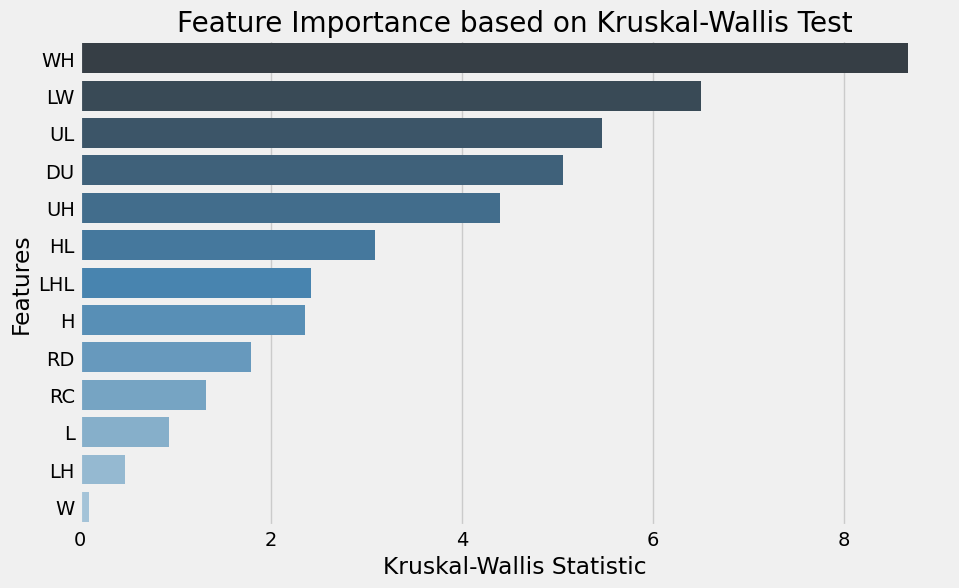
\includegraphics[width=1.0\textwidth]{figures/kw.png}
	\caption{Feature Importance Scores Using the Kruskal-Wallis Test}
	\label{fig:kw}
\end{figure}

Feature importance was assessed using the Kruskal-Wallis test, a non-parametric method that is suitable for evaluating differences in distributions across groups when the data does not follow a normal distribution. This approach was chosen because of the non-normality of the dataset and its robustness in handling continuous and ordinal data without assuming homogeneity of variances. \cite{ribeiro2024}

The analysis showed that the width-to-height ratio (WH ratio) had the highest importance score, indicating it is the most statistically significant feature for distinguishing the sex of \textit{T. granosa}. Other notable features included the length-to-width ratio (LW ratio), umbo distance-to-length ratio (UL ratio), distance between the umbos, and umbo distance-to-height ratio (UH ratio), all of which contributed significantly to the classification task.

\subsection{Performance Evaluation}

\begin{table}[H]
	\centering
	\resizebox{\textwidth}{!}{
		\begin{tabular}{lcccccc}
			\hline
			\textbf{Model} & \textbf{Accuracy (\%)} & \textbf{Precision (\%)} & \textbf{Recall (\%)} & \textbf{F1-Score (\%)} \\ \hline
			Support Vector Machine   & 58.62 & 58.62 & 58.62 & 58.44 \\
			Logistic Regression      & 57.83 & 57.83 & 57.83 & 57.61 \\
			K-Nearest Neighbors      & 51.18 & 51.31 & 51.18 & 50.77 \\
			Extra Trees              & 59.07 & 59.54 & 59.07 & 58.45 \\
			Random Forest            & 59.85 & 59.99 & 59.85 & 59.80 \\
			\cellcolor{celadon}Gradient Boosting        & \cellcolor{celadon}61.03 & \cellcolor{celadon}61.32 & \cellcolor{celadon}61.03 & \cellcolor{celadon}60.81 \\
			AdaBoost & 60.63 & 60.98 & 60.63 & 60.39 \\
			\hline
		\end{tabular}
	}
	\caption{Performance Metrics for Models with All 13 Features}
	\label{tab:performance-13-features}
\end{table}

Table~\ref{tab:performance-13-features} shows the performance metrics of different machine learning models trained using all 13 features from the dataset. Among the models, Gradient Boosting achieved the highest accuracy of 61.03\%, along with strong precision, recall, and F1-score values. AdaBoost also performed competitively, with an accuracy of 60.63\%. These results highlight the effectiveness of ensemble methods such as Gradient Boosting and AdaBoost when utilizing the full feature set, likely because of their capability to combine multiple weak learners into a more robust predictive model \cite{hussain2024}. 

\begin{table}[H]
	\centering
	\resizebox{\textwidth}{!}{
		\begin{tabular}{lcccccc}
			\hline
			\textbf{Model} & \textbf{Accuracy (\%)} & \textbf{Precision (\%)} & \textbf{Recall (\%)} & \textbf{F1-Score (\%)} \\ \hline
			Support Vector Machine   & 63.77 & 64.47 & 63.77 & 63.42 \\
			Logistic Regression      & 63.75 & 63.87 & 63.75 & 63.70 \\
			\cellcolor{celadon}K-Nearest Neighbors      & \cellcolor{celadon}64.16 & \cellcolor{celadon}64.97 & \cellcolor{celadon}64.16 & \cellcolor{celadon}63.75 \\
			Extra Trees              & 61.04 & 61.68 & 61.04 & 60.67 \\
			Random Forest            & 61.01 & 61.12 & 61.01 & 60.91 \\
			Gradient Boosting        & 64.15 & 64.24 & 64.15 & 64.01 \\
			AdaBoost                 & 61.02 & 61.26 & 61.02 & 60.82 \\
			\hline
		\end{tabular}
	}
	\caption{Performance Metrics for Models with 5 Features}
	\label{tab:performance-5-features}
\end{table}

Table~\ref{tab:performance-5-features} presents the performance of the same models using only the top 5 features identified through Kruskal-Wallis feature importance analysis. The selected features are the distance between the umbos, length-to-width ratio, width-to-height ratio, umbo distance-to-height ratio, and umbo distance-to-length ratio.

Interestingly, the overall performance of the models improved when using only the top 5 features compared to using all 13. K-Nearest Neighbors (KNN) achieved the best results with an accuracy of 64.16\%, precision of 64.97\%, recall of 64.16\%, and an F1-score of 63.75\%. Gradient Boosting followed closely behind. These findings suggest that reducing the feature set to the most relevant variables helped simplify the models, improved generalization, and enhanced predictive performance—particularly for KNN, which showed a notable improvement over its earlier results with the full feature set.

\subsection{Confusion Matrix Analysis}

\begin{figure}[!htbp]
	\centering
	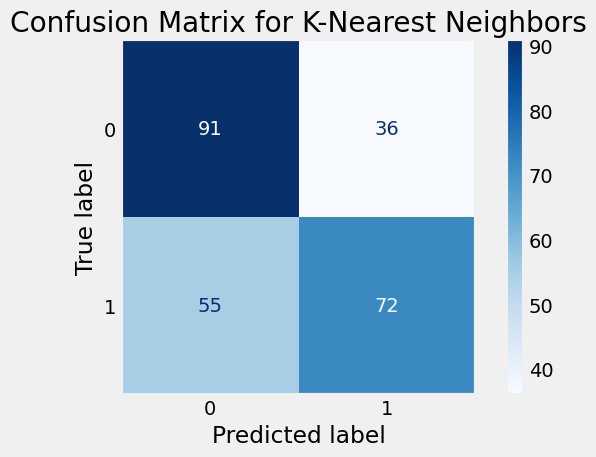
\includegraphics[width=0.8\textwidth]{figures/confusion_matrix_ml.png}
	\caption{Feature Importance Scores Using the Kruskal-Wallis Test}
	\label{fig:cm_ml}
\end{figure}

Figure~\ref{fig:cm_ml} summarizes the performance of the K-Nearest Neighbors model in classifying \Tgranosa based on their sex, where 0 represents female samples and 1 represents male samples. From the matrix, we observe that out of all the actual female samples (true label 0), 91 were correctly predicted as female (true positive for class 0), while 36 were incorrectly classified as male (false negative for class 0). On the other hand, out of all the actual male samples (true label 1), 72 were correctly predicted as male (true positive for class 1), while 55 were incorrectly classified as female (false negative for class 1).

The distribution of correct and incorrect predictions suggests that the model performs slightly better at identifying female samples compared to male samples. Nevertheless, there is a noticeable amount of misclassification in both classes, which indicates room for improvement in the model's predictive performance.